% !TEX root = ../main.tex

\begin{savequote}[99mm]
Everything starts somewhere, although many physicists disagree. But people have always been dimly aware of the problem with the start of things. They wonder aloud how the snowplough driver gets to work, or how the makers of dictionaries look up the spelling of the words. Yet there is the constant desire to find some point in the twisting, knotting, ravelling nets of space-time on which a metaphorical finger can be put to indicate that here, here, is the point where it all began\ldots
\qauthor{Terry Prattchet}
\end{savequote}

\chapter{Introduction to the theory and applications of Cellular Automata}\label{chap:intro}

We concentrate on 1D, deterministic, binary CAs with a finite number of cells, defined by a local rule with a symmetric neighborhood. Yet, the problem definition and the identification algorithm can be extended to higher dimensions and more complex state sets. Below, we give a definition of the CAs that are considered in this paper. Let $f_A\colon\{0,1\}^{2\,r+1}\to\{0,1\}$ be a function, where $r\in\mathbb{N}$, then, for any integer $N$, we define the $N$-cell global CA rule $A_N\colon\{0,1\}^N\to\{0,1\}^N$ as:
\begin{equation}
	A_N(s_1,\dotsc,s_i,\ldots,s_N) = (s_1',\dotsc,s_i',\dotsc,s_N'),
	\label{eq:glob}
\end{equation}
where $s_i' = f_A(s_{i-r},\dotsc,s_{i+r})$ and periodic boundary conditions are assumed, \emph{i.e.}\ $s_{i+N} = s_{i}$ for any $i\in\mathbb{Z}$. Such function $f_A$ will be referred to as a \emph{local rule}, while the integer $r$ will be referred to as the \emph{neighborhood radius} or simply \emph{radius}. Any local rule can be uniquely defined by a lookup table (LUT), listing all possible arguments and mapping them to the corresponding function values. The ordering of the arguments in a LUT is assumed to be lexicographic, thus only the second row needs to be stored. Therefore, a LUT will be represented as a binary vector of length $2^{2\,r+1}$. The general form of a LUT describing a local rule with unit radius ($r=1$) is shown in Table~\ref{tab:lut-example}. Note that LUTs can be used to enumerate local rules, as the coefficients $\ell_i$ can be treated as digits in the binary representation of an integer $n$, \emph{i.e.}\ the number of a local rule is given by $n=\sum_{i=1}^8 \ell_i\,2^{i-1}=(\ell_8,\ell_7,\dotsc,\ell_1)_2$. Clearly, this extends to larger radii.
\begin{table}[ht]
	\renewcommand{\arraystretch}{1.3}
	\caption{LUT of local rule $n = (\ell_8,\ell_7,\ell_6,\ell_5,\ell_4,\ell_3,\ell_2,\ell_1)_2$.}\label{tab:lut-example}
	\centering
	\begin{tabular}{|>{$}c<{$}|>{$}c<{$}|>{$}c<{$}|>{$}c<{$}|>{$}c<{$}|>{$}c<{$}|>{$}c<{$}|>{$}c<{$}|}
		\hline
		111    & 110    & 101    & 100    & 011    & 010    & 001    & 000    \\
		\hline
		\ell_8 & \ell_7 & \ell_6 & \ell_5 & \ell_4 & \ell_3 & \ell_2 & \ell_1 \\
		\hline
	\end{tabular}
\end{table}

The set of all binary sequences of finite length will be denoted by $\{0,1\}^\ast$, \emph{i.e.}\ $\{0,1\}^\ast = \bigcup_{M\in\mathbb{N}_0}\{0,1\}^M$. The function $A\colon \{0,1\}^\ast\to\{0,1\}^\ast$, satisfying $A(X) = A_M(X)$ if $X\in\{0,1\}^M$, where each of the global rules $A_M$ is defined by the same local rule, will be referred to as a \emph{generalized global rule of a CA}. Since such functions will be frequently used throughout this paper, for the sake of simplicity, we will refer to them as \emph{global rules} or \emph{rules}. In this paper, a CA is identified with its global rule. Therefore, a CA is technically a function, and by referring to a CA we refer to its global rule and vice versa.
Note that a given local rule $f_A$ uniquely defines a global rule $A$, but the opposite is not true when the radius is not fixed. For a given rule $A$, there may exist many different local rules defining it.
Fact~\ref{fac:samelocal} highlights the relationship between local rules defining the same CA.

\begin{fact}
Let $u\leq r$ be integers and let $f\colon\{0,1\}^{2\,r+1}\to\{0,1\}$ and $g\colon\{0,1\}^{2\,u+1}\to\{0,1\}$ be local rules. The CA defined by $f$ and $g$ coincide if and only if it holds that:
\begin{equation}
f(s_1,\dotsc,s_{2\,r+1}) = g(s_{r-u+1},\dotsc,s_{r+u+1})\,,
\end{equation}
for any $(s_1,\dotsc,s_{2\,r+1})\in\{0,1\}^{2\,r+1}$.\label{fac:samelocal}
\end{fact}

\begin{example}
Let the local rule $g\colon \{0,1\}\to\{0,1\}$ be defined by $g(s) = s$ (the identity) and $f\colon \{0,1\}^3\to\{0,1\}$ be defined by $f(s_1, s_2, s_3)=s_2$ (the second projection). We can see that for any $s_1, s_3\in\{0,1\}$ it holds that $f(s_1, s_2, s_3) = g(s_2) = s_2$, and thus $f$ and $g$ define the same CA, which happens to be the identity rule, but the local rules $f$ and $g$ are different.\qed
\end{example}

The set $\mathcal{A}_r$, where $r\in\mathbb{N}$ is the radius, denotes the set of all CAs that can be expressed using local rules with radius $r$. All of the CAs in $\mathcal{A}_1$ are referred to as Elementary CAs (ECAs). This class is one of the most commonly studied classes of CAs~\cite{RevModPhys.55.601}. Fact~\ref{fac:incl} shows two important properties of the sets $\mathcal{A}_r$.

\begin{fact}
	For any $r\geq 0$, $\mathcal{A}_r \subset \mathcal{A}_{r+1}$ and $\abs{\mathcal{A}_r} = 2^{2^{2\,r+1}}$.\label{fac:incl}\end{fact}

Let $A$ be a CA, $X\in \{0,1\}^M$ for some $M$ and $T\in\mathbb{N}^+$. The finite sequence of vectors given by:
\[(X, A(X), A^2(X), \dotsc, A^{T-1}(X))\,,\]
where $A^t$ denotes the $t$-th application of rule $A$, will be referred to as a \emph{space-time diagram} covering $T$ time stamps. Each of its elements will be referred to as a \emph{configuration} of the CA $A$, while the first element will be referred to as the \emph{initial configuration}. For any $t=0,1,\dotsc,T-1$ and $m=1,\dotsc,M$, $A^t(X)[m]$ denotes the state of the $m$-th cell in the $t$-th row of the space-time diagram.

\begin{example}
	We consider the four ECAs defined by local rules 40, 56, 150 and 110, whose LUTs are given in Table~\ref{tab:lut-150}. 
	Figure~\ref{fig:spatio1} depicts their corresponding space-time diagrams. All of them start from the same, random initial configuration containing 69 cells. By convention, the space-time diagrams are visualized as bitmaps in which every row corresponds to a configuration at a specific time stamp. Hence, the first row in the image is the initial configuration. Furthermore, state $1$ is visualized as a black pixel, while a white pixel corresponds to state $0$.

	\begin{figure*}
		\centering
		\subfloat[ECA 40 (Class I)]{\fbox{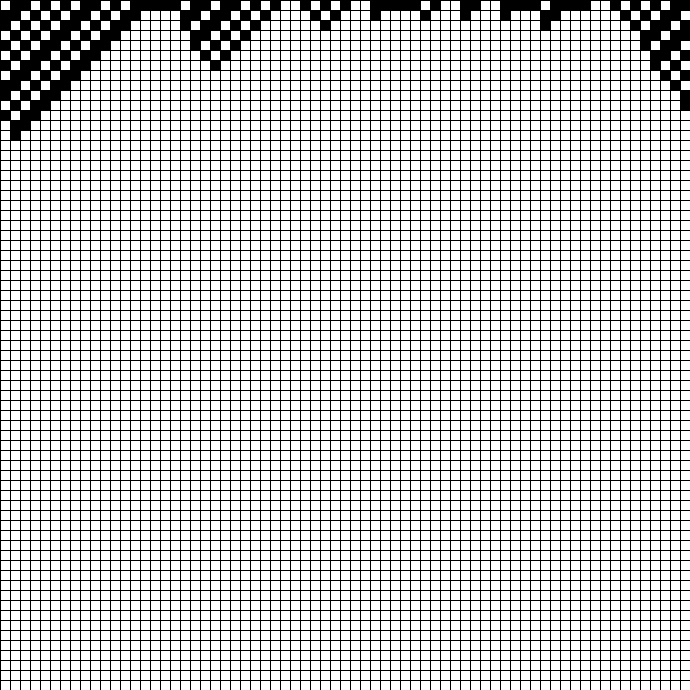
\includegraphics[width=.4\textwidth]{figs/rule-40a.png}}}\
		\subfloat[ECA 56 (Class II)]{\fbox{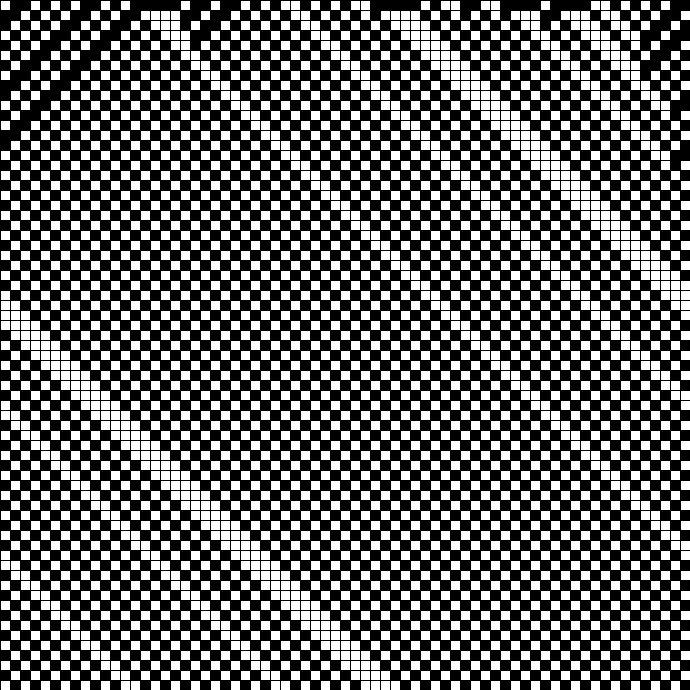
\includegraphics[width=.4\textwidth]{figs/rule-56a.png}}}\\
		\subfloat[ECA 150 (Class III)]{\fbox{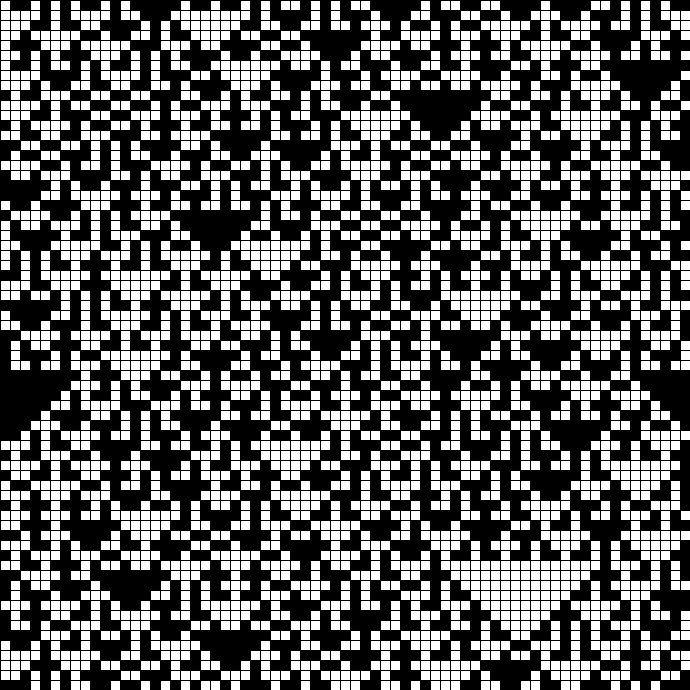
\includegraphics[width=.4\textwidth]{figs/rule-150a.png}}}\
		\subfloat[ECA 110 (Class IV)]{\fbox{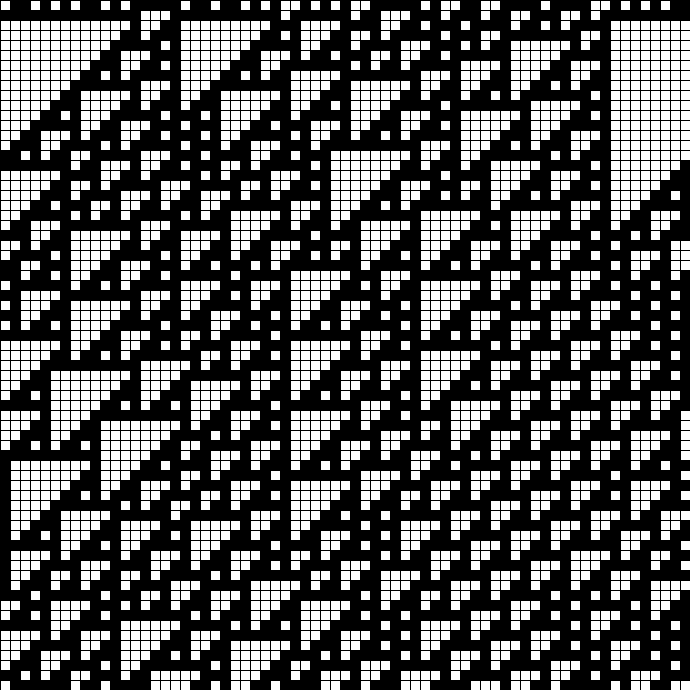
\includegraphics[width=.4\textwidth]{figs/rule-110a.png}}}
		\caption{Space-time diagrams of ECAs, containing 69 cells and 69 time stamps each, illustrating the behavioral classes that can be found among ECAs.}\label{fig:spatio1}
	\end{figure*}

	\begin{table}[ht]
	\renewcommand{\arraystretch}{1.2}
	\caption{LUTs of ECAs 40, 56, 150 and 110.}
	\label{tab:lut-150}
	\centering
	\begin{tabular}{c||>{$}c<{$}|>{$}c<{$}|>{$}c<{$}|>{$}c<{$}|>{$}c<{$}|>{$}c<{$}|>{$}c<{$}|>{$}c<{$}}
	\hline
	{\bf ECA} & {\bf 111} & {\bf 110} & {\bf 101} & {\bf 100} & {\bf 011} & {\bf 010} & {\bf 001} & {\bf 000}  \\
	\hline
	 40 & 0 & 0 & 1 & 0 & 1 & 0 & 0 & 0 \\
	\hline
	 56 & 0 & 0 & 1 & 1 & 1 & 0 & 0 & 0 \\
	\hline
	 150 & 1 & 0 & 0 & 1 & 0 & 1 & 1 & 0 \\
	\hline
	 110 & 0 & 1 & 1 & 0 & 1 & 1 & 1 & 0 \\
	\hline 
	\end{tabular}
	\end{table}
	These four ECAs exemplify the behavior that can be found among 1D two-state CAs. More precisely, Wolfram conjectures that there are four behavioral classes~\cite{RevModPhys.55.601}.  After a few time stamps, ECA 40 evolves to a homogeneous configuration (Class~I), ECA 56 reaches a periodic configuration (Class~II), ECA 150 behaves chaotically (Class~III), while ECA 110 displays complex behavior (Class~IV).\qed%
\end{example}
